
\chapter{Formal Verification of the Bitwalker Core Functionality}
\label{sec:formal-verification}

\fxfatal[inline]{improve this intro}

In this chapter we describe our work on the formal verification
of the so-called Bitwalker.
The Bitwalker shall read bit sequences from a bit stream 
and convert them to an integer. Furthermore, it shall
convert an integer into a bit sequence and write it into a bit stream.
Therefore, the Bitwalker has a read and a write function, namely \peek and \poke.

Our aim is to verify the functionality of
\peek and \poke
as well as their correct interaction.
Furthermore, we want to verify some robustness cases for \peek and \poke
and the absence of run time errors for both functions.
We won't take into account any complexity requirements.

We introduce a method to achieve these goals in section~\ref{plan}.
Moreover, it is our intention
to elaborate the method and in particular the associated tools.

Subsequently, we use the method for the functions \peek and \poke.
We provide an informal specification, an implementation and
a formal specification for each function and
present what could have been verified for the implementation.

Finally, we give an overview about the still open issues in section~\ref{issues}.


\clearpage

\section{Verification Method}
\label{plan}
\label{method}

In this section we introduce our method of choice along with the used tools.
We use a deductive verification approach to 
formally prove that a function fulfills its specification.
The foundations for deductive verification are axiomatic semantics as formulated
by Hoare~\cite{HoareCalculus}.
Figure~\ref{fig:method} shows the method with the involved verification tools.

\begin{figure}[hbt]
\centering
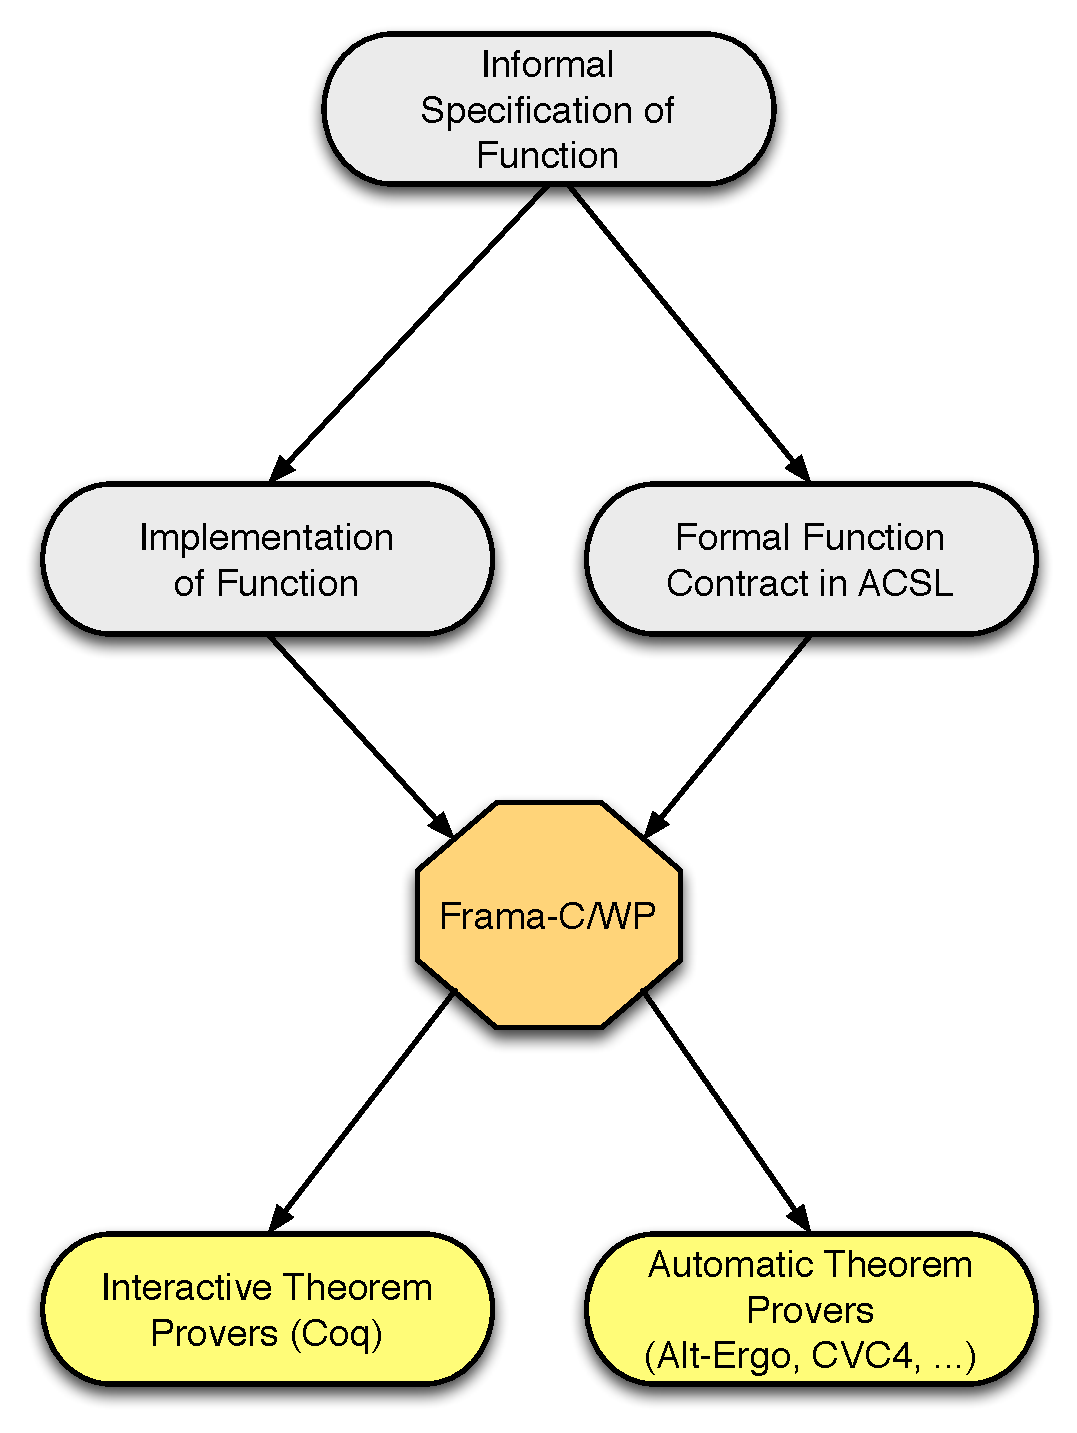
\includegraphics[width=0.60\textwidth]{figures/deductive-verification.pdf}
\caption{\label{fig:method} Deductive verification of C code with \framacwp.}
\end{figure}

Starting point is an informal specification of a function with which in mind
a implementation is written.
This informal specification is then formalized using the
\acsl specification language that is part of \framac.
The formal specification of a function is a so-called function contract
which contains preconditions to express what a function expects from its caller
and postconditions to state the guarantees after the execution.
The specification language is called 
\acsl (ANSI\slash ISO-\isoc Specification Language)~\cite{acsl} 
which is a formal language to express behavioral properties of \isoc programs.

Moreover, it is the specification language associated with 
the verification platform \framac~\cite{FramaC}
which we use along with its plug-in \framacwp~\cite{wp}.
Within \framac, the \wpframac plug-in supports
the deductive verification of \isoc programs that have been annotated with \acsl.
\framacwp generates verification conditions which are submitted to 
automatic or interactive theorem provers.
If each verification condition is discharged by at least one prover, then
the the implementation of the function satisfies its contract.

Figure~\ref{fig:method} shows that we apply the automatic
theorem provers \altergo~\cite{alt-ergo} and \cvc~\cite{cvc}
and then, if necessary, apply the interactive theorem prover \coq~\cite{Coq}
for the still unproven conditions.
Moreover, unproven conditions motivate to give some extra information
in the form of axioms, lemmas and assertions in \acsl, 
since they can ease the search of a proof.
One need to be careful with axioms because they can yield contradictions
and thus make the proof system unsound.

In order to prove the absence of run time errors we use
the \inl{rte} option of \wpframac that automatically generates \acsl
assertions for critical operations.
If all these assertions can be proven, then
the absence of run time errors is guaranteed.


\begin{framed}
The verifiers received the source code only with a high-level description
of what the Bitwalker is supposed to do.
In particular, no sufficient information about error conditions were provided.
On such a basis it is, as pointed out on Page~\pageref{lesson},
not possible to write meaningful test cases;
let alone to formally verify the functionality of the bitwalker functions.

In a first step, we therefore inspected the source code and 
derived from this an \emph{informal specification}.
This informal specification is to be understood
as a requirements document for the bitwalker functions as it should have been
available for both the programmer and the verifier.

There are several problems with this approach:
\begin{itemize}
\item
The verifier could make an error while analyzing the source code
and end up with a wrong specification. 
In fact, this happened in a first version.

\item
There could also be an error in the implementation which would then be present also
in the specification, thus leading to the claim ``the code works as implemented''.
\end{itemize}

In order to avoid these problems we submitted our informal specification
for review by the domain experts.
\end{framed}

\clearpage

\section{A First Look on \peek and \poke}

In this section we analyze the implementations of \peek 
and \poke.
The goal is to devise a more precise specification than
was original provided.
Of course, a specification derived from the source code by the verifier
must be subject to a review of the domain experts.

At his point we are already using \framacwp in order to identify
potential run time errors in the source code.

\subsection{Analysing \peek}

Listing~\ref{lst:peek-original} shows the original implementation of \peek.


\begin{listing}[hbt]
\begin{minipage}{\textwidth}
\lstinputlisting[style=acsl-block, frame=single]{./Bitwalker/Original/Bitwalker_peek.c}
\end{minipage}
\caption{\label{lst:peek-original} Original implementation of \peek}
\end{listing}

Here are some remarks on this implementation.

\begin{itemize}
\item The implementation extensively uses bit operations.
      This is of course largely a matter of taste.
      Nevertheless, it is questionable whether representing a division 
      of an index~\inl{i} by~8 as \inl{i >> 3} is better than writing it as~\inl{i/8}.
\item The argument \inl{Bitstream} represents an array that is only read.
      It is good programming practice to qualify such arguments as \inl{const}.

\item The cast of \inl{CurrentValue != 0} to \inl{uint8_t} is unnecessary for the following reasons:
\begin{itemize}
\item The result of expression \inl{CurrentValue != 0} is of type \inl{int} and has either the value~1 or~0.
\item According to the ``usual arithmetic conversions''\footnote{%
     This is indeed the heading of Section~6.3.1.8 of the C standard.
}
this value will be promoted to the type of \inl{retval << 1} which is~\inl{uint64_t}.
\end{itemize}

    Thus, the cast to \inl{uint8_t} is pointless and removing it increases the clarity of the code.

\end{itemize}

At one point, an alternative to the implementation of \peek in
Listing~\ref{lst:peek-original} was suggested.
This alternative implementation, which is shown in Listing~\ref{lst:peek-alternative}
attempts to limit the use of bit operations to a minimum.


\begin{listing}[hbt]
\begin{minipage}{\textwidth}
\begin{lstlisting}[style=acsl-block,frame=single]
  uint64_t Bitwalker_Peek (unsigned int Startposition,
                           unsigned int Length,
                           uint8_t Bitstream[],
                           unsigned int BitstreamSizeInBytes)
  {
    uint64_t retval = 0;
    for (unsigned int i = Startposition +
           BitstreamSizeInBytes*!((Startposition + Length) <=
           BitstreamSizeInBytes*8);
           i < Startposition + Length; i++)
      retval = (retval*2) +
               (uint8_t)((uint8_t)!!(Bitstream[i/8] & BitwalkerBitMaskTable[i%8]));
    return retval;
 }
\end{lstlisting}
\end{minipage}
\caption{\label{lst:peek-alternative} An alternative implementation of \peek}
\end{listing}

Interestingly, this implementation also employs unnecessary casts to \inl{uint8_t}.
However, the real problem with this alternative implementation is that it produces
different results: Calling \peek from Listing~\ref{lst:peek-original} with the arguments

\begin{verbatim}
  Startposition = 8
  Length = 32
  Bitstream[] = {254, 7, 13, 9}
  BitstreamSizeInBytes = 4
\end{verbatim}

produces~0 whereas the implementation from Listing~\ref{lst:peek-alternative} returns~118294784.
Apparently, even \peek is not so simple that its functionality can be unambiguously
understood just by looking at the code.


\clearpage

Figure~\ref{fig:peek-wp} shows a normalized representation of \peek
that is enhanced with static \acsl assertions.
These assertions can be generated by \framac for all operations where
runtime errors, that is illegal pointer accesses or arithmetic overflows, can occur.
Green bullets indicate potential runtime errors where \framacwp can verify
that they will \emph{not} occur.


\begin{figure}[hbt]
\begin{center}
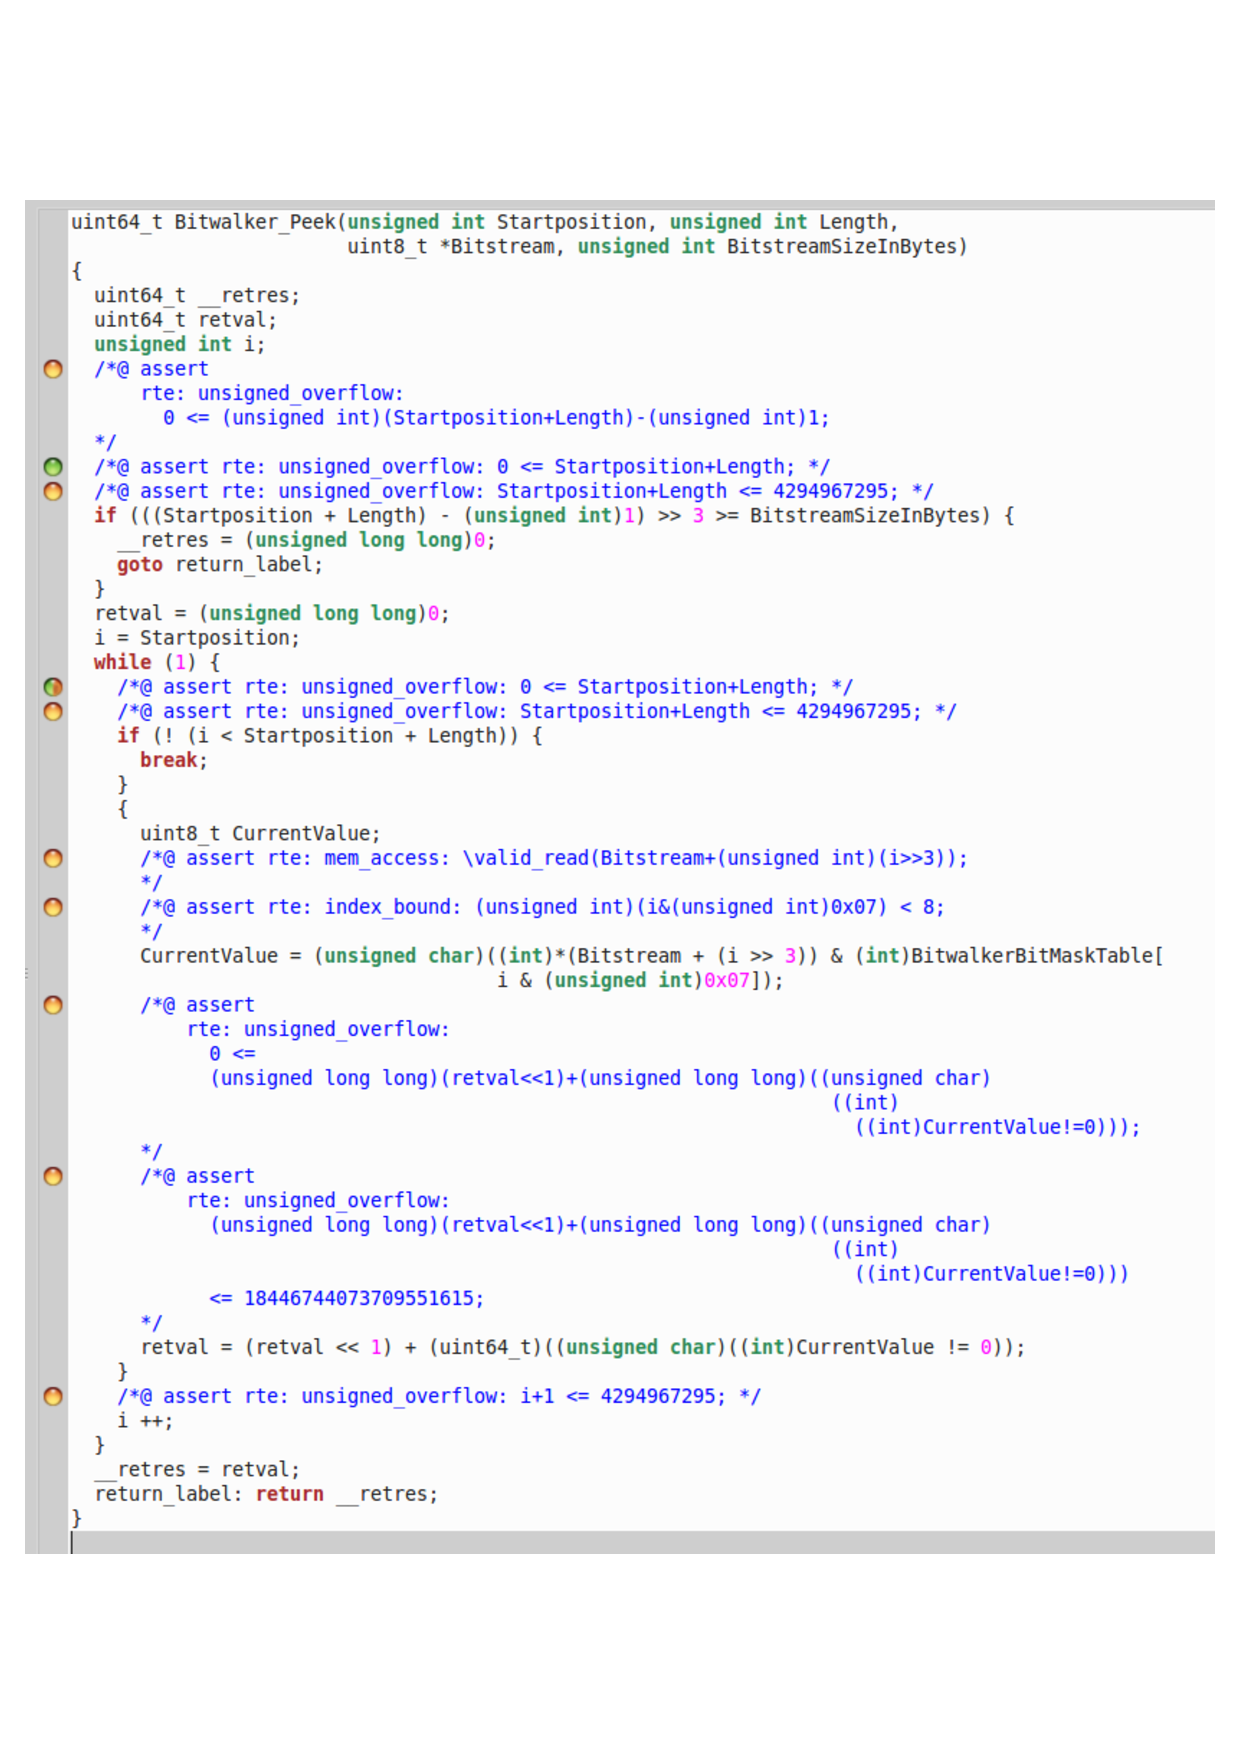
\includegraphics[width=0.95\textwidth]{figures/peek-wp.pdf}
\caption{\label{fig:peek-wp} Potential runtime errors in \peek}
\end{center}
\end{figure}

These potential runtime errors are related to the facts that at this point \framacwp
\begin{itemize}
\item cannot exclude that \inl{Length} can be greater then~64 
\item has to assume that \inl{Startposition + Length} may overflow
\item has no guarantee that \inl{BitstreamSizeInBytes} is the length 
      of the array starting at the address \inl{Bitstream}
\end{itemize}

\clearpage

\subsection{Analysing \poke}

Listing~\ref{lst:poke-original} shows the original implementation of \poke.

\begin{listing}[hbt]
\begin{minipage}{\textwidth}
\lstinputlisting[style=acsl-block, frame=single]{./Bitwalker/Original/Bitwalker_poke.c}
\end{minipage}
\caption{\label{lst:poke-original} Original implementation of \poke}
\end{listing}

Clearly visible in the code are various error conditions that are checked 
returned by~\poke.
No specifications for these error conditions have been provided.
 
\clearpage


Figure~\ref{fig:poke-wp} shows the normalized representation of \poke
with \acsl assertions that indicate potential runtime errors.

\begin{figure}[hbt]
\begin{center}
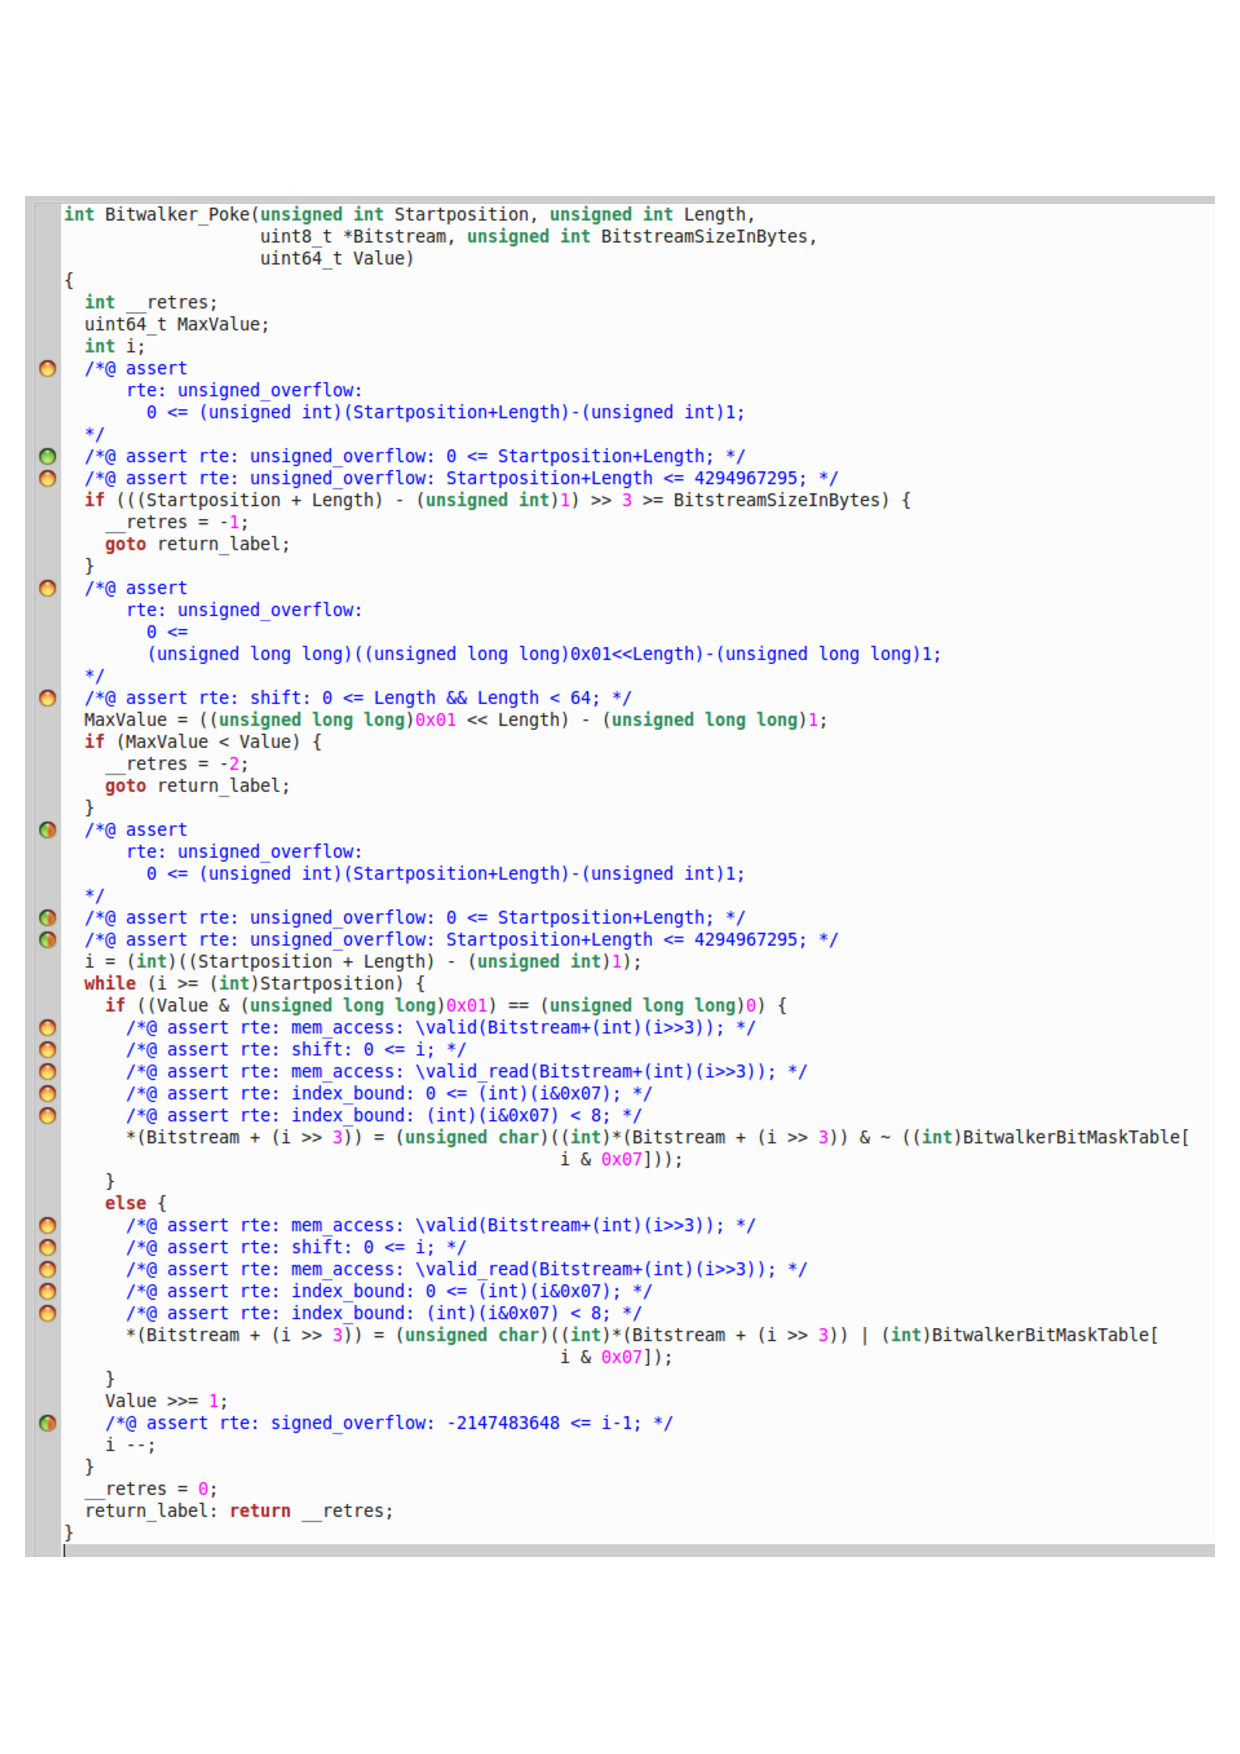
\includegraphics[width=0.99\textwidth]{figures/poke-wp.pdf}
\caption{\label{fig:poke-wp} Potential runtime errors in \peek}
\end{center}
\end{figure}

Similarly to the potential runtime errors of \peek \framacwp
faces the problem that it

\begin{itemize}
\item cannot exclude that \inl{Length} can be greater then~64 
\item has to assume that \inl{Startposition + Length} may overflow
\item has no guarantee that \inl{BitstreamSizeInBytes} is the length 
      of the array starting at the address \inl{Bitstream}
\end{itemize}

\clearpage

\section{Informal Specifications}
\label{sec:informal-specification}

Before we provide an informal specification of \peek and \poke, respectively,
we introduce some auxiliary concepts and formulate general assumptions.
We would also like to point out the following: 
When we speak of \emph{integers}, then we refer to the infinite set of mathematical
integers $\{\ldots, -1, 0, 1, \ldots\}$
and not to one of the many finite representation provided by the type system of~C.
This distinction is important because mathematical integers
usually play an important role in \acsl specifications.

\subsection{Basic Concepts}

\begin{itemize}
\item
A \emph{bit stream} is an array containing elements of type \verb"uint8_t".

A bit stream of length $n$ contains $8n$ bits.

\item
A bit stream is \emph{valid} if the array is valid.

\item 
A bit stream can be indexed both by its array indices
and its \emph{bit indices}.

Figure~\ref{fig:bitstream-indices} shows the difference between 
array indices and bit indices in a bit stream.
The two bit indices, 0~and~14,
mark bit positions in the first and second array element, respectively.

\begin{figure}[hbt]
\begin{center}
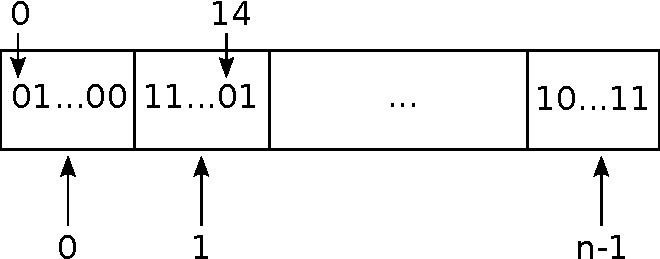
\includegraphics[width=0.40\textwidth]{figures/array_as_stream.pdf}
\caption{\label{fig:bitstream-indices} Array indices and bit indices in a bit stream}
\end{center}
\end{figure}

\item 
The C~programming language neither provides a type \emph{bit}
nor does it support random access to the bits of a bit stream.
In order to access the $i$-th bit of a bit sequence one typically
has to first access the byte with index $j = i/8$ and then access the 
bit $k = i \pmod{8}$ within this byte.
Note that in Figure~\ref{fig:bitstream-indices} 
bytes and bits are indexed in increasing order from the \emph{left}.
On the byte level, however, bits are often indexed from the \emph{right}.
For example, to access the $k$-th bit of a byte \inl{a} one can
shift this bit to the right by $7-k$ and extracts then the now
rightmost bit by performing a bit-wise \emph{and} with the value~1
%
\begin{verbatim}
   (a >> (7-k)) & 1
\end{verbatim}

\item
A \emph{bit sequence} is a consecutive sequence of bits within a bit stream
as represented in Figure~\ref{fig:bitsequence}.
\begin{figure}[hbt]
\begin{center}
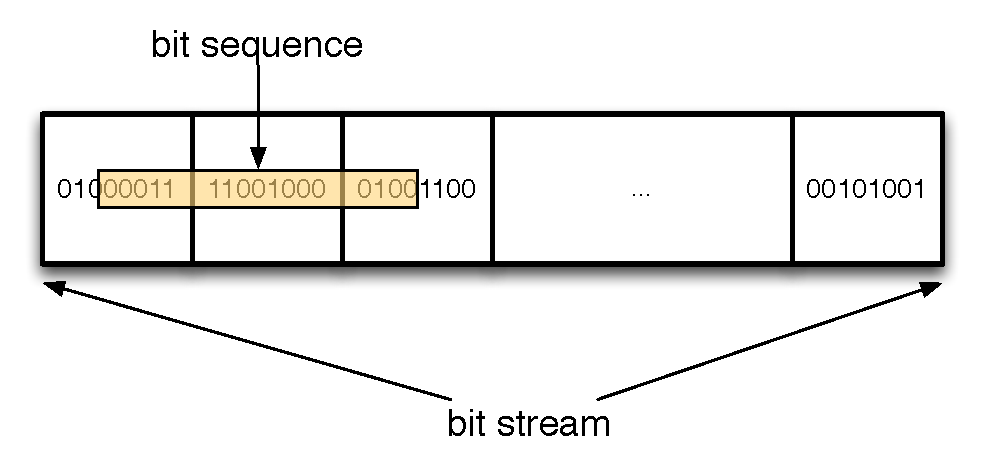
\includegraphics[width=0.40\textwidth]{figures/bit_sequence.pdf}
\caption{\label{fig:bitsequence} A bit sequence within a bit stream}
\end{center}
\end{figure}

A bit sequence is given by the position of its first bit (a bit index in the bit stream)
and its \emph{length}, that is, the number of bits it contains.

\item A bit sequence of length $l$ that starts at bit index $p$ is \emph{valid}
     with respect to a bit stream of length $n$ if the following conditions are
     satisfied
     \begin{align*}
         0 &\leq p < 8n \\
         0 &\leq p + l < 8n
     \end{align*}

\end{itemize}

We assume that the C-types \inl{unsigned int} and \inl{int}, which
are used in the implementation to represent indices, counting and error codes,
have a width of~32~bits.
We point this out here because we conducted the verification on a platform with
these characteristics.

As an aside, MISRA-C discourages the use of ``generic'' integer types
such as \inl{int} and \inl{unsigned int} and recommends the use of integer types whose names
contain the exact width.

\subsection{Informal Specification of \peek}
\label{informal-peek}

Now we specify \peek with the introduced auxiliary concepts.
The function \peek reads a bit sequence from a bit stream
and converts it to an integer.

Its function signature reads as follows:

\begin{lstlisting}[style=acsl-block]
uint64_t  Bitwalker_Peek(unsigned int Startposition, 
                         unsigned int Length,
                         uint8_t Bitstream[],
                         unsigned int BitstreamSizeInBytes);
\end{lstlisting}

\paragraph{Arguments}
The arguments of \peek have the following purpose:
\begin{itemize}
    \item \inl{Startposition} is the bit index in the bit stream 
    where the bit sequence starts.
    \item \inl{Length} is the length of the bit sequence.
    \item \inl{Bitstream} is the array which provides the bit stream.
    \item \inl{BitstreamSizeInBytes} is the length of the array 
    containing the bit stream. 
\end{itemize}

\paragraph{Preconditions}
The following preconditions shall hold for the function arguments.
Note that additional constraints are implicitly expressed by the use
of \emph{unsigned} integer types.

\begin{itemize}
\item \inl{Bitstream} is a valid array of length \inl{BitstreamSizeInBytes}

\item \inl{Length} $\leq$ \inl{64} and

\item \inl{Startposition} $\leq$ \inl{UINT_MAX} - \inl{Length}.
      This condition expresses that no arithmetic overflows shall occur
      when evaluating \inl{Startposition + Length}.
\end{itemize}

\paragraph{Description}
As mentioned, the function \peek reads a bit sequence from a bit stream
and converts it to a 64-bit unsigned integer.

For a bit sequence $(b_0, b_1,\ldots,b_{n - 1})$ the function \peek returns the sum
\begin{align}
\label{eq:peek-result}
    \sum_{i=0}^{n-1} b_i \cdot 2^{(n - 1) - i} 
\end{align}

Note that is a higher-level description than what is done in the source code.
There is, in our opinion, not much point to reflect all of the low-level bit operations
into the specification if a clearer description is at hand.

If the bit sequence is not valid, then \peek shall return~0.
We were wondering why the implementation maps an illegal input to a legitimate output.
The code providers argued along the lines that this error condition was not
considered important enough to be properly reported.
One can interpret this design decision as an attempt to increase the
robustness of the function against illegal values.
In general, we recommend to explicitly describe all error conditions
and to devise a consistent error detection and error recovery strategy.


\subsection{Informal Specification of \poke}

In this section we examine the function \poke
in the same manner as we did it for \peek.

The function \poke converts an integer to a bit sequence and writes it
into a bit stream.
Its function signature reads as follows:
\begin{lstlisting}[style = acsl-block]
int      Bitwalker_Poke(unsigned int Startposition,
                        unsigned int Length,
                        uint8_t Bitstream[],
                        unsigned int BitstreamSizeInBytes,
                        uint64_t Value);
\end{lstlisting}


\paragraph{Arguments}
The arguments have the following purpose:

\begin{itemize}
    \item \inl{Startposition} is the bit index in the bit stream 
    where the bit sequence starts.
    \item \inl{Length} is the length of the bit sequence.
    \item \inl{Bitstream} is the array which provides the bit stream.
    \item \inl{BitstreamSizeInBytes} is the length of the array 
    containing the bit stream. 
    \item \inl{Value} is the integer which shall be converted into a bit sequence.
\end{itemize}


\paragraph{Preconditions}
The following conditions shall hold for the function arguments:

\begin{itemize}
\item \inl{Bitstream} is a valid array of length \inl{BitstreamSizeInBytes}

\item \inl{Startposition + Length} is less than \verb"UINT_MAX".
\end{itemize}

Note that additional constraints are implicitly expressed by the use
of \emph{unsigned} integer types.


\paragraph{Description}
Now we can specify \poke as follows:
The function \poke converts a 64-bit unsigned integer to a bit sequence and 
writes it into a bit stream.

For $0 \leq x$ exists a shortest sequence of~0 and~1
$(b_0, b_1,\ldots,b_{n - 1})$
such that
\begin{align}
    \sum_{i=0}^{n-1} b_i \cdot 2^{(n - 1) - i} = x.
\end{align}

The function \poke tries to store the sequence $(b_0, b_1,\ldots,b_{n - 1})$
in the bit sequence of \inl{Length} bits that starts
at bit index \inl{Startposition}.

The return value of \poke depends on the following three cases:

\begin{itemize}
\item 
If the bit sequence is valid, then there are two cases:

\begin{itemize}
\item
If \inl{Length} is greater or equal than $n$, then  the sequence
$(\overbrace{0,\ldots,0}^{\mathtt{Length}-n},b_0, b_1,\ldots,b_{n - 1})$
is stored in the bit stream starting at \inl{Startposition}.
The return value of \poke is 0.

\item
If \inl{Length}  is less then $n$, then the
sequence $(b_0, b_1,\ldots,b_{n - 1})$ cannot be stored and\\
\poke returns~$-2$.
\end{itemize}

\item 
If the bit sequence is not valid, then \poke returns~$-1$.
\end{itemize}

\clearpage

\section{Tests for \peek and \poke}

In this section we show some tests for \peek and \poke.
These tests were derived from the informal specification in 
Section~\ref{sec:informal-specification}.

We use the \CC\ class \inl{boost::dynamic_bitset} in order to represent
\inl{bit sequences} in our tests.
This class\footnote{
  See \url{http://www.boost.org/doc/libs/1_55_0/libs/dynamic_bitset/dynamic_bitset.html}
},
which is part of the \textsf{Boost} libraries,
provides a higher-level and easier to use interface to bit sequences than is possible in~C.

Specifically, we use in our \CC\ test code the following typedefs

\begin{lstlisting}[style = acsl-block]
  typedef std::vector<uint8_t>           Bytestream;

  typedef boost::dynamic_bitset<uint8_t> Bitstream;
\end{lstlisting}

to represent arrays of sequences of bytes and bits, respectively.
An object of type \inl{Bitstream} can be initialized with an object
of type \inl{Bytestream}. The type \inl{Bitstream} offers random access
to its stored bits.
In addition, it allows to
\begin{itemize}
\item  compute the unsigned value represented in the bit stream by calling the
       method \inl{to_ulong()}, thereby representing the functionality of \peek
\item  create a bit stream from an unsigned integer value by a special constructor,
       thus representing the functionality of \poke
\end{itemize}

Listings~\ref{lst:test_peek} and~\ref{lst:test_poke} show fragments of our test code
for \peek and \poke, respectively.

While testing the Bitwalker was not our main objective it proved useful for
the following reasons.

\begin{itemize}
\item It helped us formulating the formal specifications of \peek and \poke.
  
\item It allowed us to quickly detect that the alternative implementation of
      \peek in Listing~\ref{lst:peek-alternative} is not equivalent to the
      original implementation in Listing~\ref{lst:peek-original}.

\item It provided some assurance that our re-implementations of \peek and \poke
      that we use in Section~\ref{sec:formal-specification} do not behave differently
      than the original implementations.
\end{itemize}

\clearpage

\begin{listing}[hbt]
\begin{minipage}{\textwidth}
\lstinputlisting[style=acsl-block, frame=single]{./Bitwalker/Tests/test_peek.cpp}
\end{minipage}
\caption{\label{lst:test_peek} Test code for \peek}
\end{listing}

\clearpage

\begin{listing}[hbt]
\begin{minipage}{\textwidth}
\lstinputlisting[style=acsl-block, frame=single]{./Bitwalker/Tests/test_poke.cpp}
\end{minipage}
\caption{\label{lst:test_poke} Test code for \poke}
\end{listing}

\clearpage

\section{Formal Specification with \acsl}
\label{sec:formal-specification}

In this section we discuss formal contracts for \peek and \poke.
The contracts are written in \acsl.
Note that the contracts do not provide a full formal specification
of the functionality of the respective functions.
As of now they describe the main operation modes and are aimed at showing
that no runtime errors can occur if the functions are called 
in a context where their preconditions are satisfied..

\subsection{Formal Specification of \peek}
\label{sec:formal-specification-peek}


Listing~\ref{lst:spec-peek} shows an \acsl contract with the 
main operation modes of \peek.
Note that we have labeled various properties of the contract.
This feature of \acsl allows us to refer to them more easily.
Note also that we sometimes use shorter names than in the original implementation.

\begin{listing}[hbt]
\begin{minipage}{\textwidth}
\lstinputlisting[style=acsl-block, frame=single]{./Bitwalker/Modified3/Bitwalker_Peek.h}
\end{minipage}
\caption{\label{lst:spec-peek} Formal specification of \peek in \acsl}
\end{listing}

The structure of this contract is as follows:

\begin{description}
\item[General preconditions an assigns clauses]~

\begin{itemize}
\item
The property \inl{valid_bitstream} expresses that 
\inl{Bitstream} is the starting address of a valid array of length
\inl{BitstreamSize}.

\item
The property \inl{valid_length} expresses the requirement that only
bit sequences with a length less than~64 are to be read.

\item
The two \inl{overflow} properties request that no arithmetic overflow
shall occur for the expressions \inl{Start + Length} and
\inl{8 * BitstreamSize}, respectively.

Given the operational context of the \bitwalker these overflows are unlikely
to happen. 
Nevertheless, a formal verification tool such as \framacwp does not
know about the size of ETCS telegrams and therefore needs this information.

\item
The assigns clause expresses that \peek will not change any memory location
outside its scope.
This means in particular that \peek will not have side effects.
      
\end{itemize}

\item[Behavior for invalid bit sequences]~

The behavior \inl{bit_sequence_too_long} describes the situation where
the specified bit sequence does not fit into the underlying bit stream.

\begin{itemize}
\item
The assumes clause describes the conditions to which this behavior applies.
Note that we use the formulation 
\begin{verbatim}
   (Start + Length) > 8 * BitstreamSize
\end{verbatim}
in order to describe an invalid bit sequence whereas the original implementation
in Listing~\ref{lst:peek-original} used the expression
\begin{verbatim}
   ((Start + Length - 1) >> 3) >= BitstreamSize
\end{verbatim}

The main difference is that we reformulate the division inherent in the shift
operation as a multiplication.
Moreover, switching to a strict inequality saves us the trouble
to deal with a potential overflow in the term \inl{(Start + Length - 1)}
that occurs if both \inl{Start} and \inl{Length} are~0.
Last but no least, the new expression is also shorter.

\item
The postcondition of this behavior is that \peek is expected to return~0.
Not surprisingly, we also request that no external memory locations are
changed when this behavior is active.

\end{itemize}

\item[Behavior for valid bit sequences]~

The behavior \inl{normal_case} describes the normal operation mode of \peek.
\begin{itemize}
\item
Note that the assumes clause is the negation of the assumes clause  of
the behavior~\inl{bit_sequence_too_long}.

\item
Again we specify that no assignments are to occur.

\item 
At this point the formalization of the behavior of \peek is incomplete.
We only specify, the rather weak postcondition, that now overflow shall occur
when computing the result.
The complete formalization, which must be based on Formula~\eqref{eq:peek-result}
on Page~\pageref{eq:peek-result}, will be part of a later release this document.
\end{itemize}

\item[Relationship of both behaviors]~

The specification contains also statements about the relationship
of the behaviors \inl{bit_sequence_too_long} and \inl{normal_case}.

\begin{itemize}
\item
The clause \inl{complete behaviors} expresses that
the assumptions of both behaviors cover all admissible 
input values according to the general preconditions.

\item
The clause \inl{disjoint behaviors} expresses
that there are no input values that fit both 
behaviors.
\end{itemize}

These clauses, which support the writing complete and non-contradictory specifications,
will be checked \framacwp.
\end{description}

\clearpage

\subsection{Loop Invariant for \peek}

Listing~\ref{lst:impl-peek} shows our modified version of \peek.
There are several reasons for these modifications:

\begin{itemize}
\item Loop invariants and static assertions had to be inserted into
      the source code to support the verification.
\item Some shift operations were rewritten as divisions\slash multiplications
      to be more similar to the specification.
\item We felt that the slightly shorter variable names make the source code
      better legible.
\end{itemize}

\fxfatal{need assurance that implementation does change its behavior}

\begin{listing}[hbt]
\begin{minipage}{\textwidth}
\lstinputlisting[style=acsl-block, frame=single]{./Bitwalker/Modified3/Bitwalker_Peek.c}
\end{minipage}
\caption{\label{lst:impl-peek} Implementation of \peek with \acsl loop invariants}
\end{listing}

\clearpage

\subsection{Formal Specification of \poke}
\label{sec:formal-specification-poke}

Finally, the behavior \inl{normal} assumes 
that \inl{Value} is not too big and the bit sequence is valid. 
Here, \poke writes the particular bit sequence into \inl{Bitstream} 
while all other memory locations are unaltered.
For all behaviors there is one postcondition to state what
the return value shall be in this case.


\begin{listing}[hbt]
\begin{minipage}{\textwidth}
\lstinputlisting[style=acsl-block, frame=single]{./Bitwalker/Modified3/Bitwalker_Poke.h}
\end{minipage}
\caption{\label{lst:spec-poke} Formal Specification of \poke}
\end{listing}


\clearpage

\subsection{Loop Invariants for \poke}

\begin{listing}[hbt]
\begin{minipage}{\textwidth}
\lstinputlisting[style=acsl-block, frame=single]{./Bitwalker/Modified3/Bitwalker_Poke.c}
\end{minipage}
\caption{\label{lst:impl-poke} Implementation of \poke with loop invariants}
\end{listing}

\clearpage

\section{Formal Verification with \framacwp}
\label{sec:verification}
\label{verification-peek}

\fxfatal{not ready for review}

In this section we present the current state of the verification results 
for \peek.
Table~\ref{tab:results-peek} discriminates the results for
three different types of verification conditions (VCs).

\begin{table}[hbt]
  \centering
  \begin{tabular}[htb]{lccc}
    \toprule
     & \# VC & Proven VCs & Verification rate in \%\\
    \midrule
    lemmas & 1 &0 & 0 \\
    %\midrule
    rte-assertions&9&5&55\\
    rest &18 &17&94\\
 %   \bottomrule
%    &27&22&81\\
    \bottomrule
  \end{tabular}
  \caption{Verification Results of \peek}
  \label{tab:results-peek}
\end{table}


The first row contains the lemmas we used to ease the verification for the automatic theorem provers.
The second row contains the \inl{rte}-assertions 
concerning the absence of run time errors.
The third row shows all other verification conditions for \peek
which are mainly about functional behavior.
However, they also contain the postconditions for the robustness cases
and the loop specification.

For each row we listed the total number of generated verification conditions,
the number of proven verification conditions and the verification rate
that is the percentage of proven verification conditions. 

The verification rate for the \inl{rte}-assertions are very low 
due to the difficulty for \framac to deal with bit operations.
In order to increase this rate, we will verify the absence
of run time errors separately and will provide additional lemmas and axioms
to ease the verification.
We point out some of the related challenges in section~\ref{issues}.



In this section we present the current state of verification results of 
for \poke.
The results are shown in Table~\ref{tab:results-poke}.
 We listed the different verification conditions 
 row by row like we did for \peek.

The function \poke has significantly more unproven verification conditions than \peek
this is because it is more complex and alters memory locations via bit operations.
Therefore, we will verify the absence of run time errors separately as well.

\begin{table}[hbt]
  \centering
  \begin{tabular}[h]{lccc}
    \toprule
     & \# VC & Proven VCs & Proven VCs in \%\\
    \midrule
    lemmas & $1$ &$0$ & $0$ \\
    %\midrule
    rte-assertions&$19$&$7$&$36$\\
    rest &$49$ &$38$&$77$\\
    %\bottomrule
    %&$68$&$45$&$66$\\
    \bottomrule
  \end{tabular}
  \caption{Verification Results of \poke}
  \label{tab:results-poke}
\end{table}

\clearpage

\section{Open Issues}
\label{issues}

\fxfatal{not ready for review}


We have seen in this section that \wpframac currently does not deal very well with bit operations.
This is due to the fact that \wpframac's memory models do not provide 
much information about bit operations.
As a consequence, the provers have few options to manipulate the proof goal.
This problem is known and \cealist is working on a solution for the next release of \wpframac.

As a workaround one could introduce axioms which provide
additional facts about bit operations. 
The problem with using axioms is that one can easily introduce wrong facts
which lead to contradictions making the whole proof system unsound. 
Thus, this approach requires a careful review of the added axioms.

Moreover, the chosen automatic theorem provers are generally not very
good when it comes to mixing arithmetic and bit operations.
There is, however, an automatic theorem prover, namely \z,
which can handle arithmetic and bit operations, using a specific syntax.
\framac's interface for \z does not currently takes advantage of this, 
but this may change in a future release.
We therefore expect a better automatic verification rate for the verification of BitWalker.

Another approach to deal with unproven verification conditions consists in
applying an \emph{interactive theorem prover} such as \coq.
Using \coq's rich support for proof manipulation would certainly be very helpful
for the discharge of more proof obligations.

